\documentclass{article}
\usepackage[utf8]{inputenc}
\usepackage{amsmath}
\usepackage{amssymb}
\usepackage{amsfonts}
\usepackage{amssymb}
\usepackage{minted}
\usepackage{graphicx}
\usepackage{algorithm}
\usepackage{algorithmic}
\graphicspath{ {img/} }
\usepackage{titlesec}
\usepackage[a4paper,margin=1in,footskip=0.25in]{geometry}
\usepackage{fancyhdr}
\pagestyle{fancy}
%basic page layout

%draw finite state machine
\usepackage{tikz}
\newcommand{\hwnumber}{11}
\newcommand{\Lcvy}{\mathcal{L}}
%header and footer settings
\lhead{Algorithms and Data Structure \hwnumber}
\chead{Yiping Deng}
\rhead{\today}

\titlelabel{\thetitle\enspace}

\begin{document}
\title{Algorithms and Data Structure \hwnumber}
\author{Yiping Deng}
\maketitle
\thispagestyle{fancy}
\section*{Problem 1}
Such algorithm is obviously incorrect. 
Consider a graph with loop such that the
sum of the loop is negative. Including the loop one more time will lead to a even lower path,
thus we can conclude that if there is a negative loop, there is no shortest path.
Example is given below:\\
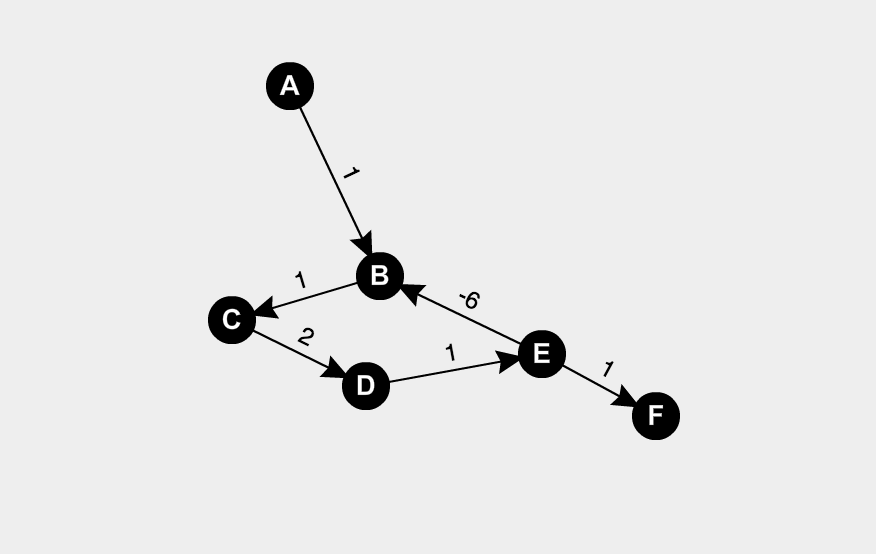
\includegraphics[width=\textwidth]{g1.png} \\
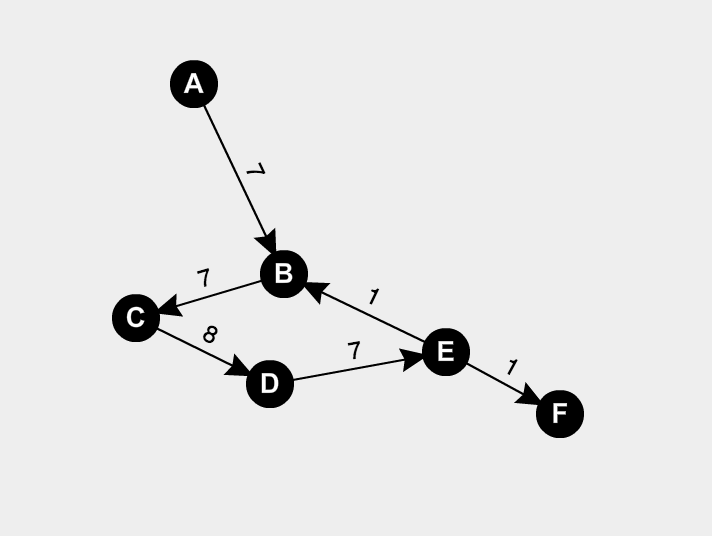
\includegraphics[width=\textwidth]{g2.png}

\section*{Problem 2}
\inputminted{python}{p2.py}
\section*{Problem 3}
\subsection*{a)}
Let's first rephase our problem in math.

Let $G = (V, E)$ to be a directed graph such that
every pair $u, v \in V, u \neq v$, either $(u, v) \in E$ or
$(v, u) \in E$ is satisfied, but not all. Then there exists a finite sequence $(v_i)_{i \in \mathbb{N}}$
formed by set $V$ such that $(v_i, v_{i + 1}) \in E$.

Proof: 
The base case with $|V| = 2$ is trivial. There is only
two possibility. $(v_1, v_2) \in E$ or $(v_2, v_1) \in E$.
Each case we can generate a Hamiltonian path.

Suppose the statement holds for $|V| = n$, consider
$|V'| = n + 1$. Pick $v_0 \in V'$, define subgraph
defined on $W = V' - {v_0}$. There is a ordering of $W$, denoted
$w_1, ..., w_n$. Define $m = max(\{i:\forall j \leq i. (v_j, v_0) \in E \})$.

If such $m$ is not well defined, we can place $v_0$ at the beginning,
forming $v_0, w_1, w_2, ..., w_n$ as a Hamiltonian path.

If $m$ is well defined, we can place $v_0$ as following:
$$w_1, w_2, ..., w_m, v_0, w_{m + 1}, ..., w_n$$

\subsection*{b)}
\inputminted{python}{p3.py}
\end{document}
